\clearpage
\setcounter{page}{1}
\maketitlesupplementary


% \section{Rationale}
% \label{sec:rationale}
% % 
% Having the supplementary compiled together with the main paper means that:
% % 
% \begin{itemize}
% \item The supplementary can back-reference sections of the main paper, for example, we can refer to \cref{sec:intro};
% \item The main paper can forward reference sub-sections within the supplementary explicitly (e.g. referring to a particular experiment); 
% \item When submitted to arXiv, the supplementary will already included at the end of the paper.
% \end{itemize}
% % 
% To split the supplementary pages from the main paper, you can use \href{https://support.apple.com/en-ca/guide/preview/prvw11793/mac#:~:text=Delete%20a%20page%20from%20a,or%20choose%20Edit%20%3E%20Delete).}{Preview (on macOS)}, \href{https://www.adobe.com/acrobat/how-to/delete-pages-from-pdf.html#:~:text=Choose%20%E2%80%9CTools%E2%80%9D%20%3E%20%E2%80%9COrganize,or%20pages%20from%20the%20file.}{Adobe Acrobat} (on all OSs), as well as \href{https://superuser.com/questions/517986/is-it-possible-to-delete-some-pages-of-a-pdf-document}{command line tools}.

\section{Implementation details of VisTex-DINO and other comparison methods}

We also implemented VisTex-OVLM on GroundingDINO-T \cite{liu2023groundingdino}, denoted as VisTex-DINO. The MSTB design mirrors that of VisTex-GLIP, employing two "fully connected (fc) + ReLU" layers. Based on the feature size and scale extracted by the pre-trained GroundingDINO-T's vision encoder, $H$ is set to 100. Since the intermediate features of GroundingDINO have $W$ values that vary with image size, we applied bilinear interpolation to also set $W$ to 100. GroundingDINO's intermediate features are available at three scales, making $M=3$. MSTB is applied to both the image backbone and the feature enhancer of GroundingDINO-T, with max pooling across stages used for non-parametric multi-stage fusion. All other training settings are consistent with those of VisTex-GLIP.

% 至于正文中comparison methods，We used recent top-performing approaches for comparison, adopting published results where available and reproducing results with recommended settings on PASCAL VOC and MSCOCO when needed. 需要说明的是，为了公平比较，其中OWL-ViT和OWL-ViT v2使用的权重版本分别是"CLIP ViT-L/14"和“CLIP B/16 ST+FT”，因为这两个权重在预训练过程中没有刻意剔除MSCOCO和LVIS中可能出现的类别，接近于我们使用的OVLM的权重的预训练设置。
\textcolor{red}{For the comparison methods, we selected recent top-performing approaches, adopting published results where available and reproducing results with recommended settings on PASCAL VOC and MSCOCO when necessary. Notably, to ensure a fair comparison, the weights used for OWL-ViT and OWL-ViT v2 are "CLIP ViT-L/14" and "CLIP B/16 ST+FT," respectively. These weights were chosen because they were not specifically trained to exclude categories that might appear in MSCOCO or LVIS, making their pre-training settings closer to those of the OVLM weights we used.}

\section{Performance on ODinW13 subsets}

Following \cref{sec:4.4} of the main text, we provide detailed transfer results on the ODinW13 subsets \cite{li2022glip} in \cref{tab:odinwresult}. ODinW13 \cite{li2022odinw} is composed of 13 subsets from ODinW35, spanning specialized natural domains such as aquarium species, surgical instruments, and aerial imagery, among others. Although the categories in these 13 datasets may appear in the pre-training dataset of OVLM, their performance results still, to some extent, reflect the model's capability in real-world scenarios. The specifics of ODinW13 are outlined in \cref{tab:odinwsetting}. All methods, including ours, were trained on the MSCOCO base set, treating downstream task sets as novel sets and evaluating them with 2-shot support images. The results are presented in the table below. These results further validate VisTex-OVLM's superior transferability across diverse domains, demonstrating its robustness and adaptability in handling significant domain shifts.

% Following \cref{sec:4.4} of the main text, we provide the detailed transfer results on ODinW13 subsets \cite{li2022glip} in \cref{tab:odinwresult}.  ODinW13 \cite{li2022odinw} 是ODinW35的13个子集构成， spans 13 specialized natural domains, such as aquarium species, surgical instruments, and aerial imagery, etc. 尽管这13个数据集中的类别可能出现在OVLM的预训练数据集中，在他们上面的表现结果仍然在某些程度上可以展现模型在real-world scenario下的表现。 The specifics of ODinW13 are outlined in \cref{tab:odinwsetting}. All methods, including ours, were trained on the MSCOCO base set, treating downstream task sets as novel sets and evaluating them with 2-shot support images. The results are presented in the table below. These results further validate VisTex-OVLM's superior transferability across diverse domains, demonstrating its robustness and adaptability in handling significant domain shifts.

\begin{table}[h]
    \centering
    \resizebox{\columnwidth}{!}{
    \renewcommand\arraystretch{1}
    \begin{tabular}{c|cccc}
    \hline
    \textbf{Dataset} & \textbf{Objects of interest} & \textbf{Train} & \textbf{Val} & \textbf{Test} \\ \hline
    PascalVOC & Common objects (PascalVOC 2012) & 13690 & 3422 & \textbackslash{} \\
    AerialDrone & Boats, cars, etc. from drone images & 52 & 15 & 7 \\
    Aquarium & Penguins, starfish, etc. in an aquarium & 448 & 127 & 63 \\
    Rabbits & Cottontail rabbits & 1980 & 19 & 10 \\
    EgoHands & Hands in ego-centric images & 3840 & 480 & 480 \\
    Mushrooms & Two kinds of mushrooms & 41 & 5 & 5 \\
    Packages & Delivery packages & 19 & 4 & 3 \\
    Raccoon & Raccoon & 150 & 29 & 17 \\
    Shellfish & Shrimp, lobster, and crab & 406 & 116 & 58 \\
    Vehicles & Car, bus, motorcycle, truck, and ambulance & 878 & 250 & 126 \\
    Pistols & Pistol & 2377 & 297 & 297 \\
    Pothole & Potholes on the road & 465 & 133 & 67 \\
    Thermal & Dogs and people in thermal images & 142 & 41 & 20 \\ \hline
    \end{tabular}
    }
    \caption{The objects of interest for each subset and the image number of each split in ODinW13.}
    \label{tab:odinwsetting}
\end{table}

\begin{table*}[t]
    \centering
    \resizebox{\textwidth}{!}{
    \renewcommand\arraystretch{1}
    \begin{tabular}{c|ccccccccccccc|c}
    \hline
    \textbf{Method} & \textbf{AerialDrone} & \textbf{Vehicles} & \textbf{Aquarium} & \textbf{Mushrooms} & \textbf{Raccoon} & \textbf{Packages} & \textbf{Pothole} & \textbf{Shellfish} & \textbf{Rabbits} & \textbf{Pistols} & \textbf{Egohands} & \textbf{Pascalvoc} & \textbf{Thermal} & \textbf{Mean} \\ \hline
    \textbf{Meta-DETR} & 16.5 & 32.5 & 18.2 & 36.1 & 34.2 & 31.4 & 22.8 & 28.2 & 36.6 & 34.1 & 35.2 & 30.1 & 37.1 & 30.2 \\
    \textbf{DiGeo} & 22.6 & 37.3 & 25.1 & 49.2 & 41.4 & 44.2 & 26.7 & 39.8 & 47.0 & 38.7 & 41.6 & 42.2 & 39.7 & 38.1 \\
    \textbf{DeFRCN} & 23.5 & 36.4 & 24.8 & 43.8 & 44.1 & 44.9 & 25.6 & 40.1 & 45.3 & 39.0 & 43.5 & 50.9 & 35.4 & 38.3 \\
    \textbf{MFD} & 24.5 & 38.7 & 29.4 & 46.2 & 45.1 & 50.1 & 28.4 & 38.4 & 48.4 & 43.5 & 46.3 & 50.5 & 42.2 & 40.9 \\
    \textbf{MQ-Det} & 21.2 & 36.5 & 30.0 & 45.3 & 41.1 & 41.6 & 28.3 & 37.5 & 46.9 & 44.1 & 39.7 & 48.4 & 40.3 & 38.5 \\
    \textbf{VisTex-GLIP} & \textbf{27.4} & \textbf{41.2} & \textbf{33.3} & \textbf{50.7} & \textbf{46.7} & \textbf{55.2} & \textbf{30.1} & \textbf{46.0} & \textbf{49.6} & \textbf{51.1} & \textbf{55.9} & \textbf{51.2} & \textbf{47.8} & \textbf{45.1} \\ \hline
    \end{tabular}
    }
    \caption{Detailed 2-shot transfer results on ODinW13 subsets. The best values are highlighted in \textbf{bold}.}
    \label{tab:odinwresult}
\end{table*}

\section{More ablation and visualization results}

\subsection{Ablation on shot fusion mode}
\textcolor{red}{When integrating multiple shot features, there are various fusion modes available. \cref{tab:shotfus} presents the performance of different fusion approaches. Experimental results indicate that concatenation yields the best results, as it maximally preserves the information from all shots, thereby preventing information loss. Support samples provide detailed semantic guidance for query prediction, and concatenation allows the model to maintain the unique information of each shot while utilizing data from multiple support samples. This method helps GLIP better grasp the support sample distribution for query prediction, enhancing performance.}

\begin{table}[t]
    \centering
    \resizebox{0.7\linewidth}{!}{
    \begin{tabular}{c|ccc}
    \hline
    \multirow{2}{*}{\textbf{Shot Fusion Mode}} & \multicolumn{3}{c}{\textbf{2-shot}} \\ \cline{2-4} 
     & \textbf{AP} & \textbf{bAP} & \textbf{nAP} \\ \hline
    \textbf{element-wise addition} & 41.6 & 41 & 41.9 \\
    \textbf{max} & 48.5 & 48.4 & 48.6 \\
    \textbf{average} & 47.9 & 45.2 & 48.1 \\
    \textbf{concat} & \textbf{50.3} & \textbf{48.6} & \textbf{51.8} \\ \hline
    \end{tabular}
    }
    \caption{Ablation on shot fusion mode. Best results are marked in \textbf{bold}.}
    % \vskip -0.08in
    \label{tab:shotfus}
\end{table}

\subsection{Ablation on MSF}
\textcolor{red}{MSF’s innovation is its efficient use of OVLM’s multi-stage object-text alignment without extra parameters. \cref{tab:stagefus} in the main text shows multi-stage fusion’s effectiveness. We conducted an MSF ablation study in \cref{MSF} using different common fusion methods. Max pooling outperforms other non-parametric fusion methods. This is because max pooling can highlight the most informative features across stages while reducing the negative impact of redundant noise.}

\begin{table}[h]
% \vspace{-10pt}
% \vspace{-10pt}
\centering
\label{MSF}
\resizebox{0.7\columnwidth}{!}{
    \begin{tabular}{c|ccc}
    \hline
    \multirow{2}{*}{\textbf{Stage Fusion Mode}} & \multicolumn{3}{c}{\textbf{2-shot}} \\ \cline{2-4} 
     & \textbf{AP} & \textbf{bAP} & \textbf{nAP} \\ \hline
    \textbf{element-wise Addition} & 36.7 & 37.4 & 31.6 \\
    \textbf{max} & \textbf{50.3} & \textbf{48.6} & \textbf{51.8} \\
    \textbf{average} & 46.8 & 48.3 & 41.4 \\
    \textbf{concat} & 39.4 & 39.3 & 39.4 \\ \hline
    \end{tabular}
}
\caption{Ablation on MSF. Best results are marked in \textbf{bold}.}
% \vspace{-13pt}
\end{table}


\subsection{Ablation on image prompt engineering}
\begin{table}[t]
    \centering
    \resizebox{0.7\linewidth}{!}{
    \begin{tabular}{c|c}
    \hline
    \multirow{2}{*}{\textbf{Engineering Method}} & \textbf{2-shot} \\ \cline{2-2} 
     & \textbf{AP} \\ \hline
    \textbf{baseline} & 16.3 \\
    \textbf{BG blur} & \textbf{49.6} \\
    \textbf{dye object red in grays image} & 19.5 \\
    \textbf{add red object outline} & 28.3 \\
    \textbf{crop} & 44.2 \\
    \textbf{crop large context} & 30.8 \\ \hline
    \end{tabular}
    }
    \caption{Ablation on image prompt engineering methods. “Baseline” indicates directly inputting the original image. "crop" means cropping out the target region based on ground truth bounding box while "crop large context" enlarges ground truth bounding box by $k=10$ pixels. "BG blur" technique applies a shadow (intensity of 0.1) and Gaussian noise (kernel size of 15 and a standard deviation of 3) to the background area. Best results are marked in \textbf{bold}.}
    \label{tab:Iengineer}
\end{table}

This ablation study (\cref{tab:Iengineer}) followed the same experimental setup outlined in the main text: (1) Conducted on VisTex-OVLM in a 2-shot setting on MSCOCO using GLIP-L; (2) mAP was reported for both base and novel classes, with all other settings kept optimal. Several methods for preprocessing and inputting image prompts were tested, following CLIPSeg \cite{luddecke2022clipseg} settings unless specified. Experimental results show that the "BG blur" technique performs best. It highlights the target object while preserving some background, unlike "crop" and "baseline." Additionally, it avoids overlaying original image pixels, preventing information loss.

\subsection{Attention heatmaps}

We present a series of attention heatmaps (\cref{fig:heatmap}) illustrating the effects of different prompting modes and key components, corresponding to the methods described in \cref{tab:ab-prompting} of the main text. These heatmaps visualize object feature attention relative to text features. For "VisTex-GLIP without text prompt", the heatmap represents attention exclusively to textualized visual tokens.

The heatmaps reveal that GLIP-FF and GLIP-MAPLE exhibit notable noise attention in non-object background areas. While MQ-Det effectively suppresses background noise, its attention on target objects is less focused. In contrast, VisTex-GLIP demonstrates superior focus on target objects while significantly reducing noise attention. Notably, the attention heatmap for VisTex-GLIP without text prompt shows weaker focus on targets compared to its counterpart using text prompt. This observation underscores the importance of text prompt in providing essential semantic guidance, which crucially influences OVLMs’ object-text alignment and overall performance.

\begin{figure}
    \centering
    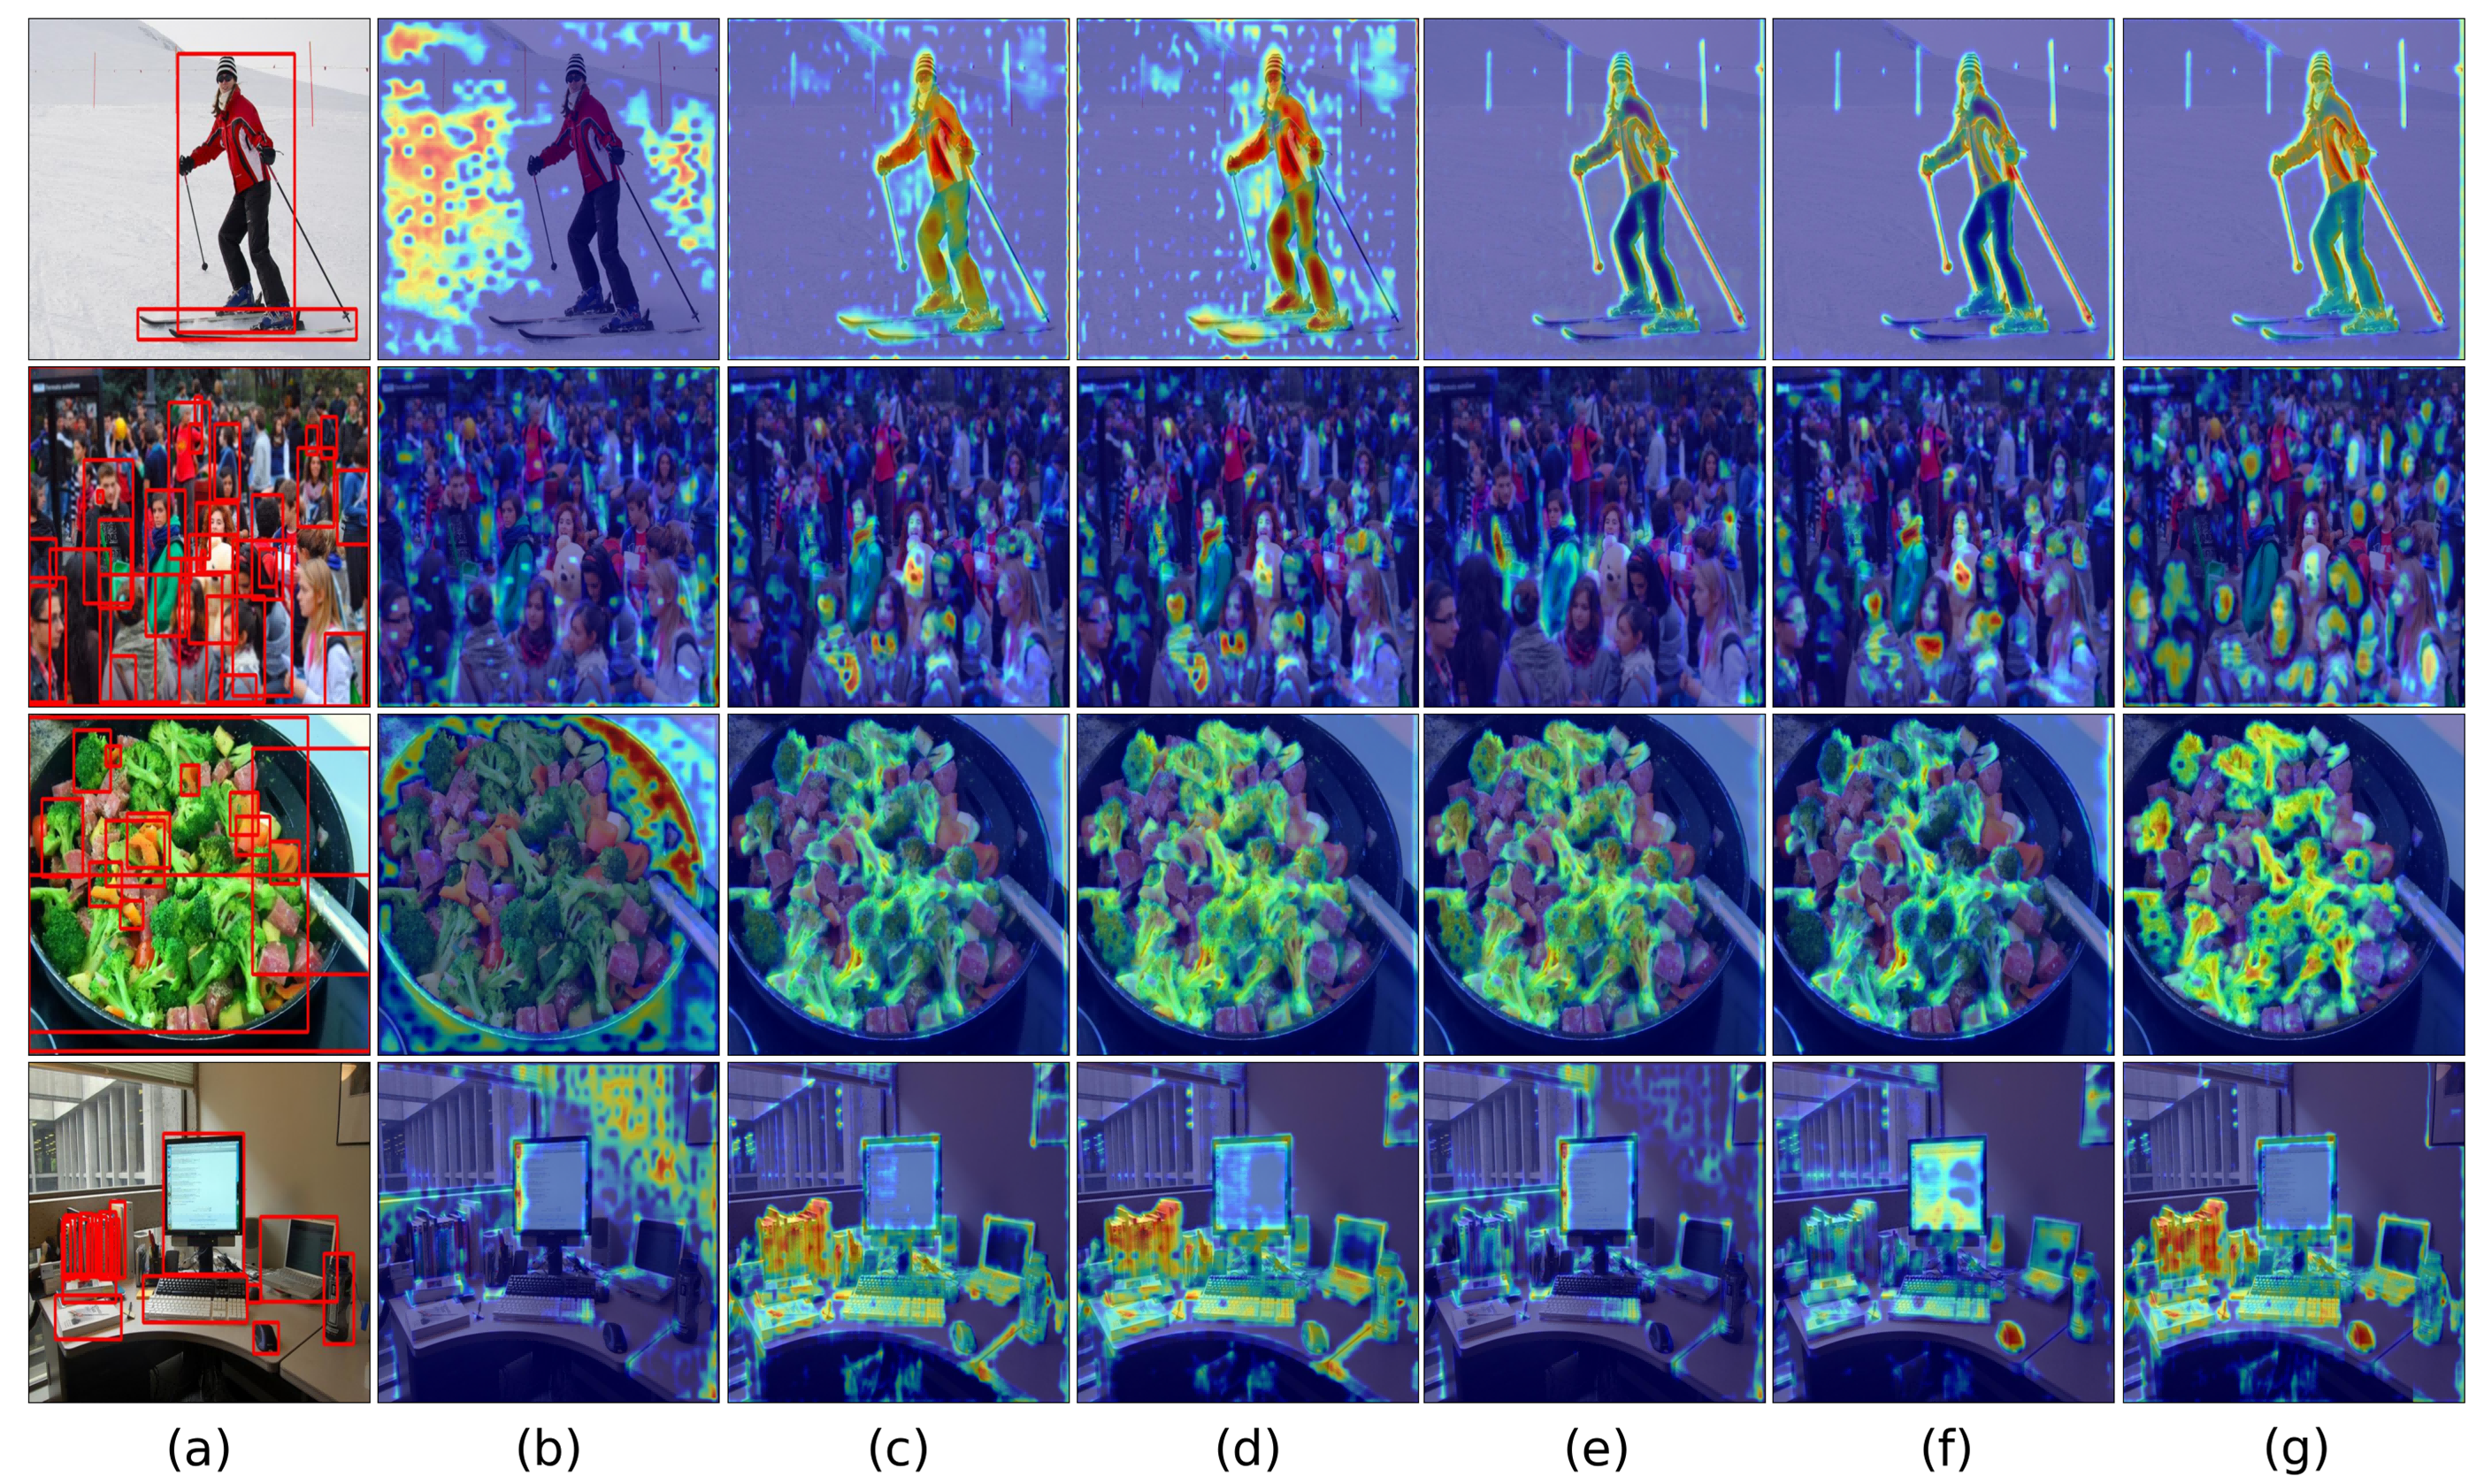
\includegraphics[width=\linewidth]{corr_attentionmap.png}
    \caption{Attention heatmaps illustrating the effects of different prompting modes and key components. (a) Ground truth, (b) GLIP-ZS (zero-shot), (c) GLIP-FF (fully fine-tuning), (d) GLIP-MaPLe, (e) MQ-Det, (f) VisTex-GLIP without text prompt, (g) VisTex-GLIP.}
    \label{fig:heatmap}
\end{figure}

\subsection{More output visualization}

We provide 10-shot output examples for VisTex-GLIP on PASCAL VOC in \cref{fig:pascal}. The settings are corresponded to \cref{tab:pascal-com} in the main text.

\begin{figure}[h]
    \centering
    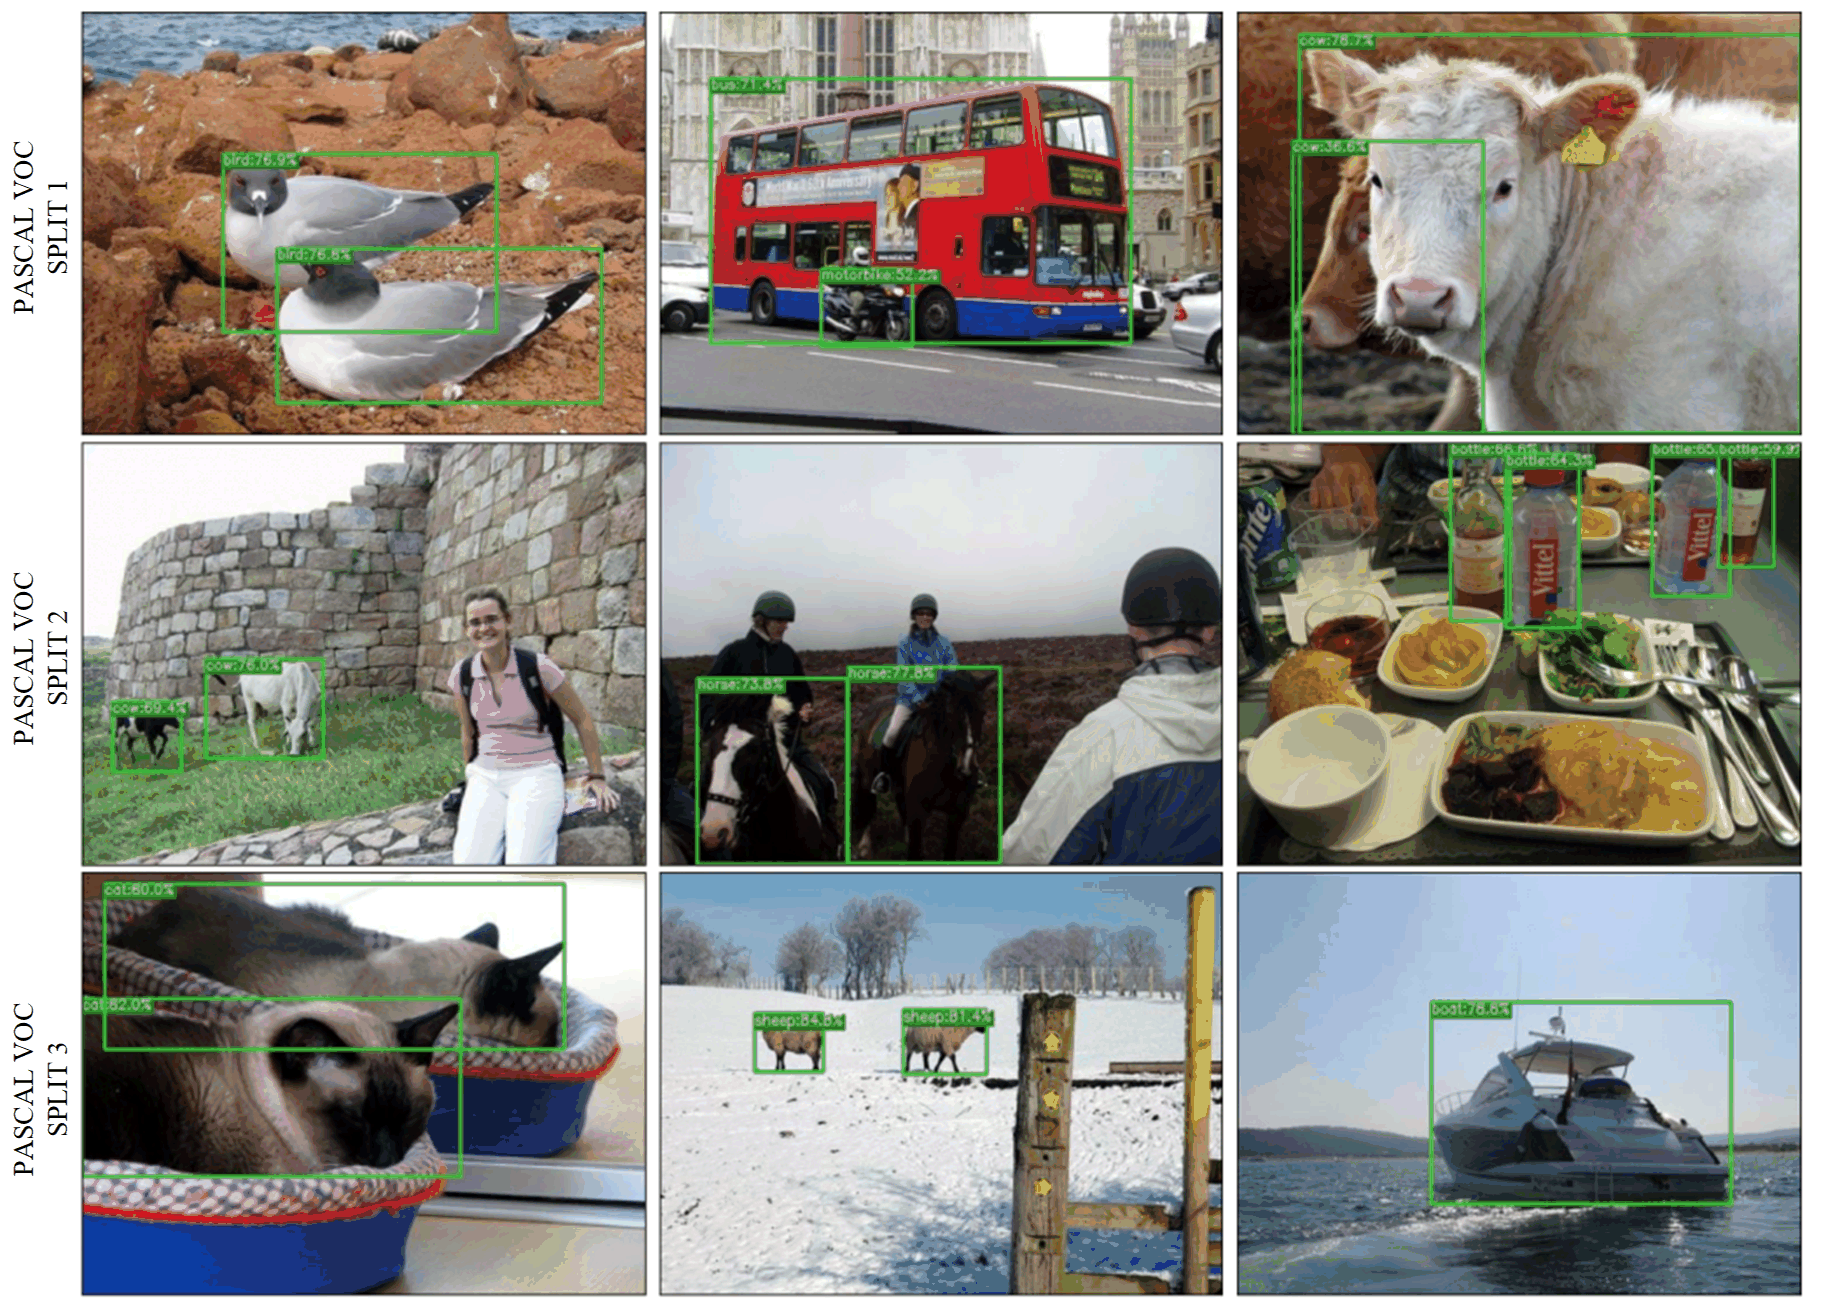
\includegraphics[width=\linewidth]{PASCAL VOC.png}
    \caption{Visualization of VisTex-GLIP’s 10-shot object detection results on PASCAL VOC. For simplicity, only detections of novel-class objects are illustrated. The settings are corresponded to \cref{tab:pascal-com} in the main text.}
    \label{fig:pascal}
\end{figure}


\begin{figure}[t]
    \centering
    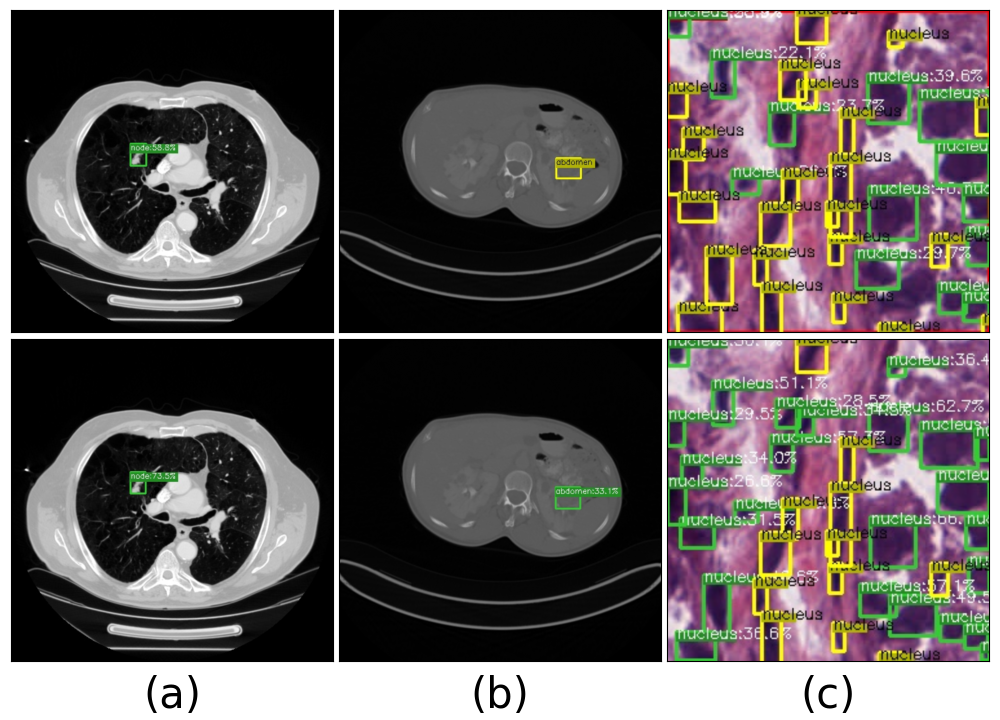
\includegraphics[width=\linewidth]{medical.png}
    \caption{Output visualizations for medical datasets. The first row illustrates the inference results when models trained solely on the MSCOCO base set were directly applied to the medical datasets. The second row demonstrates results after briefly fine-tuning the MSTB in a 2-shot setting on the medical tasks. (a) LIDC, (b) Deepleision, (c) MoNu. Green, red, and yellow boxes denote true positives, false positives, and false negatives. }
    \label{fig:med}
\end{figure}

\begin{figure}[t]
    \centering
    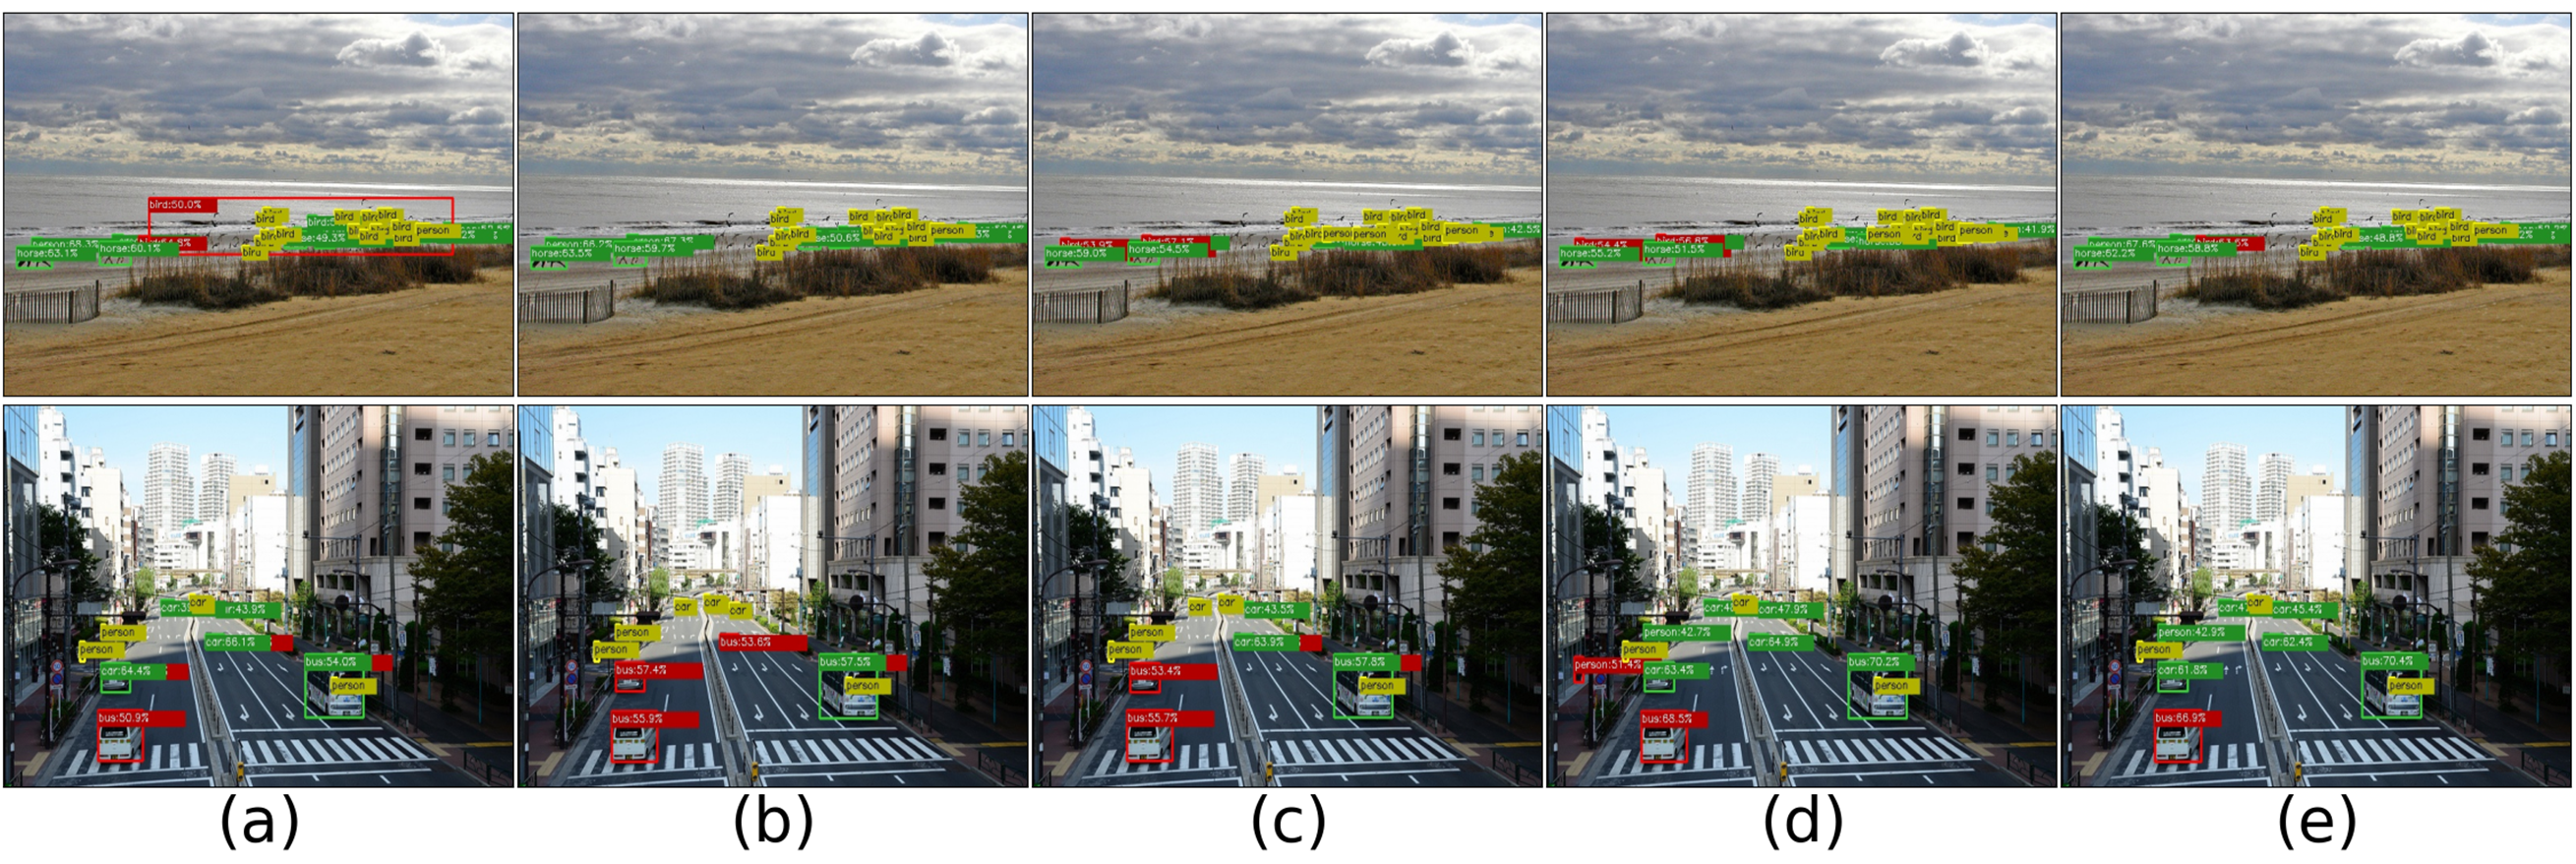
\includegraphics[width=\linewidth]{failure.png}
    \caption{Failure cases. (a) GLIP-ZS, (b) GLIP-FF, (d) GLIP-MaPLe, (e) MQ-Det, (f) VisTex-GLIP. Green, red, and yellow: true positives, false positives, and false negatives.}
    % 
    \label{fig:failure}
\end{figure}

\section{Output visualization for real-world downstream tasks}

\cref{fig:odinw} and \cref{fig:med} present the output visualizations for real-world downstream tasks, including ODinW13 subsets and medical datasets (MoNu, LIDC, and Deeplesion).

The visualizations in \cref{fig:odinw} adhere to the settings described in \cref{sec:4.4} of the main text, where all methods, including ours, were trained on the MSCOCO base set. Downstream task sets were treated as novel sets, and evaluations were conducted using 2-shot support images, directly showcasing inference results on novel classes.

\cref{fig:med} focuses on datasets with larger domain gaps, specifically medical datasets. The first row illustrates the inference results when models trained solely on the MSCOCO base set were directly applied to the medical datasets. The second row demonstrates results after briefly fine-tuning the MSTB in a 2-shot setting on the medical tasks.

\textcolor{red}{We also provide some failure cases of our method on natural images in \cref{fig:failure}. As shown, these failures primarily occur in scenarios with dense or small objects, which is similar to the challenges observed in medical images in \cref{fig:med}. We attribute this limitation to the weak representation of small objects in the pre-trained OVLM and the inherent difficulty of fitting novel category distributions with limited support samples. Addressing these issues will be a focus of future research.}

% 我们还在图18中给出了一些我们的方法在自然图像的failure cases。可以看到，这些failure primarily occur in scenarios with dense or small objects. 这和 \cref{fig:med}中展示的医学图像的状况类似。我们认为这个limitation源于pre-trained OVLM细小物体表征姣弱，以及少量support samples本身难以拟合novel categories 的distribution。如何解决这些问题将是未来的研究方向。



\begin{figure*}
    \centering
    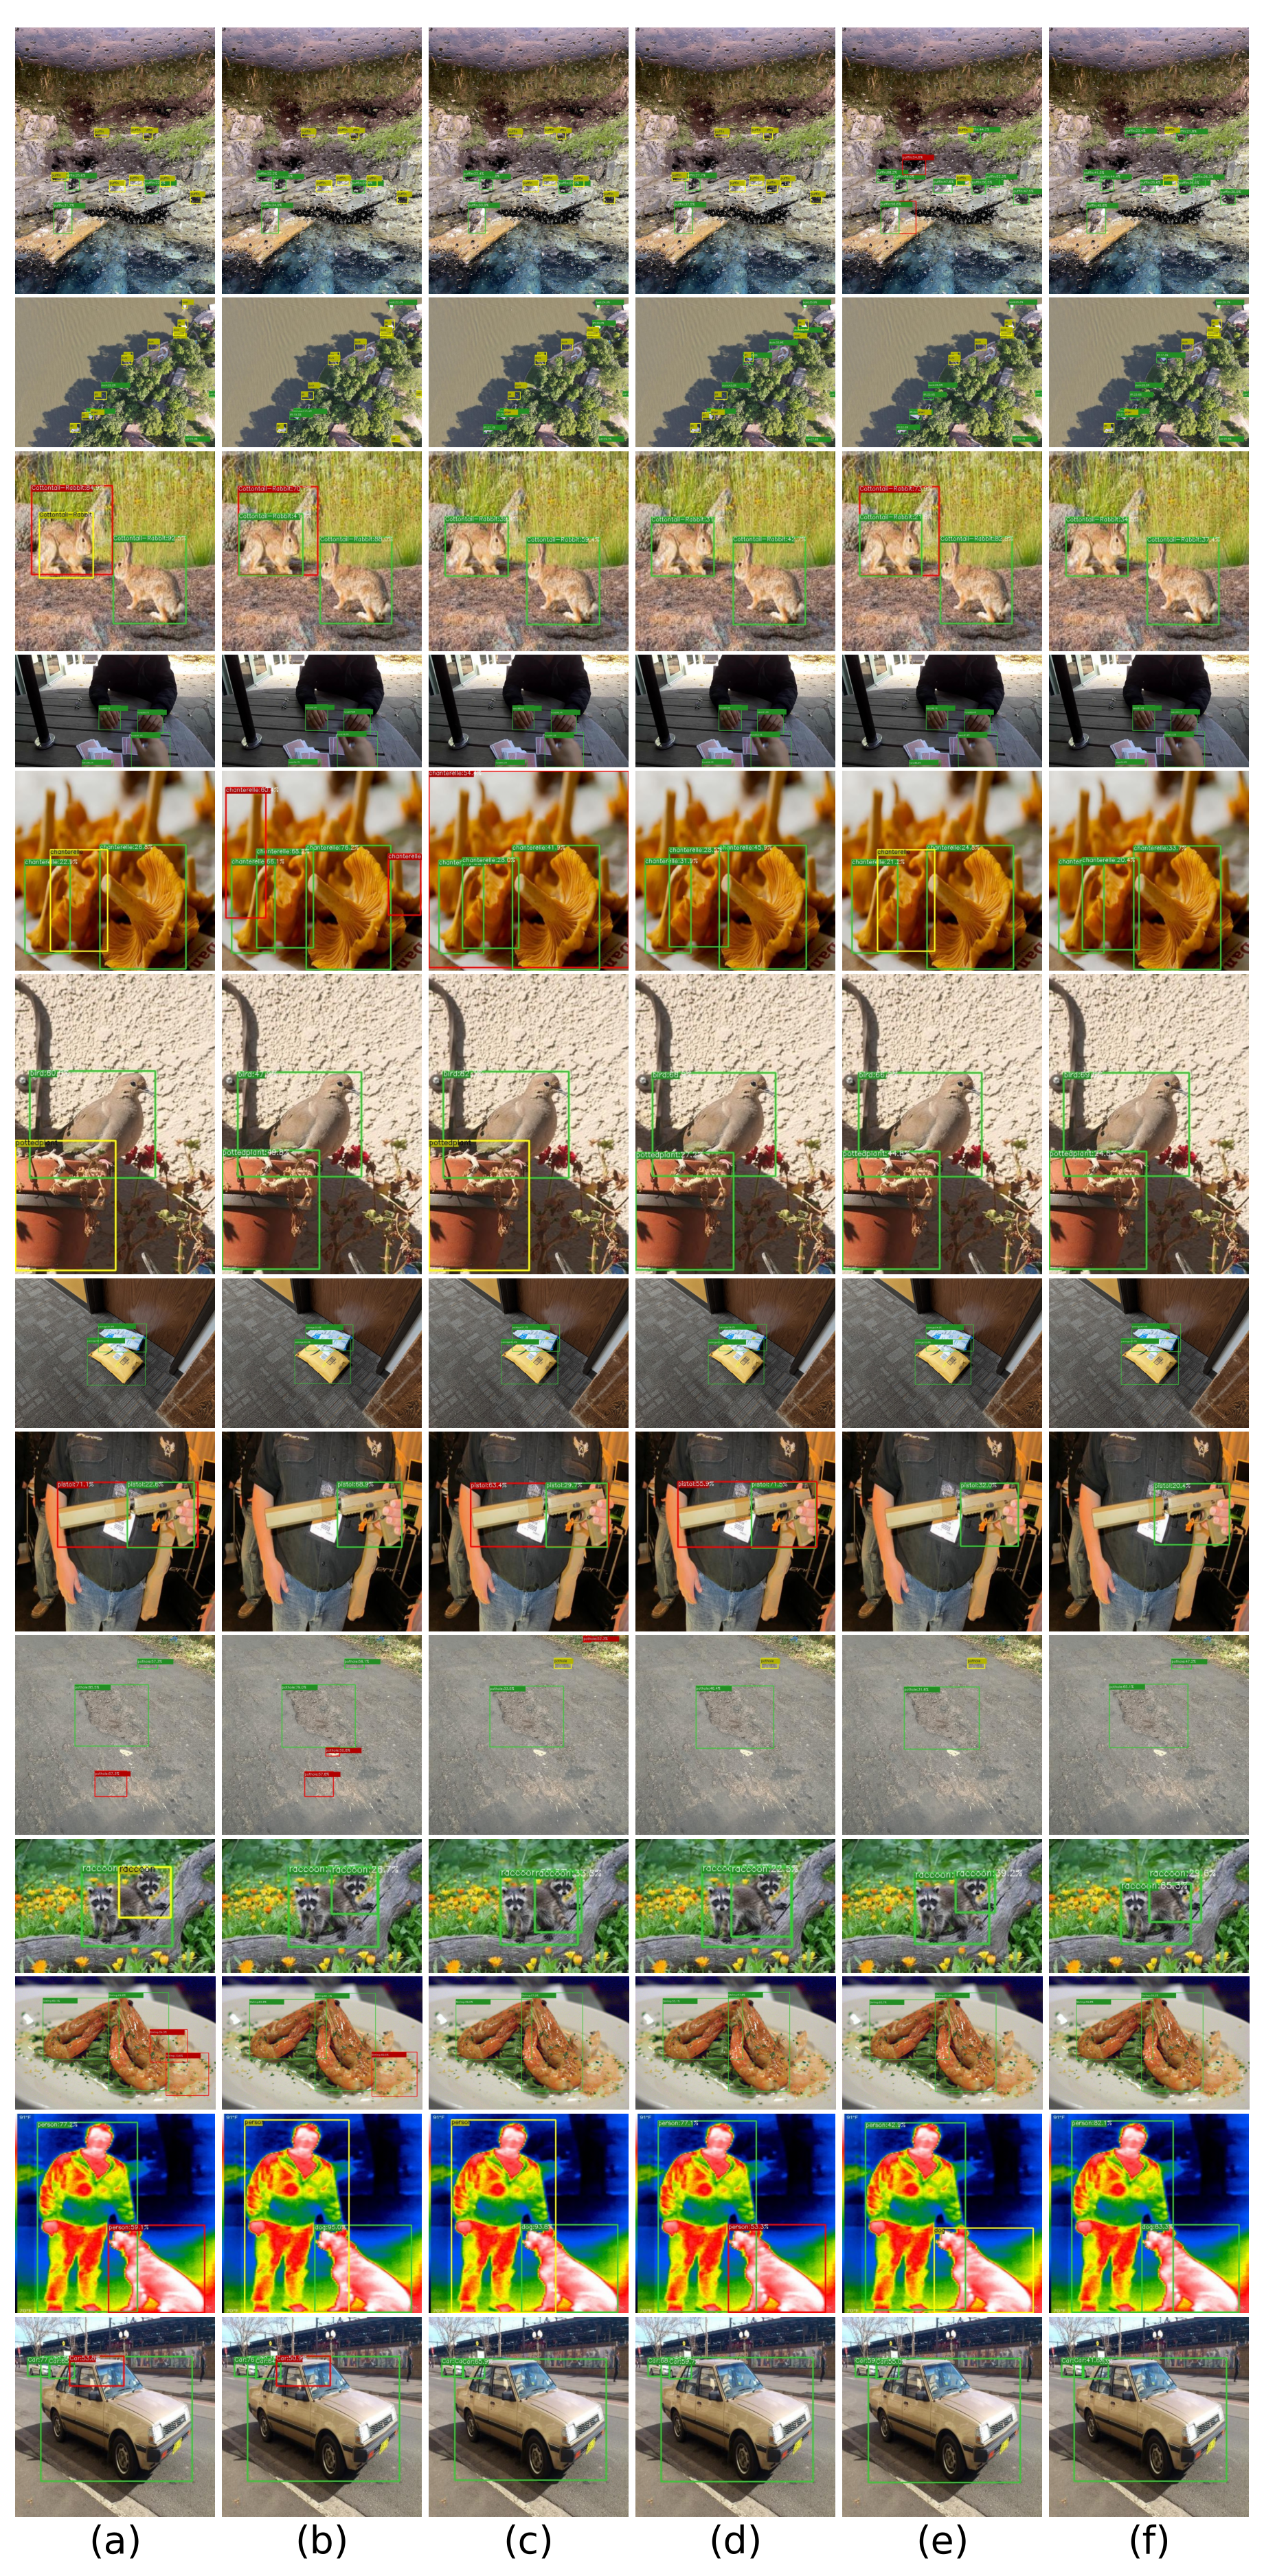
\includegraphics[width=0.61\textwidth]{ODinW13_sd.png}
    \caption{Comparison output visualizations on ODinW13. From top row to the bottom: Aquarium, AerialDrone, Rabbits, EgoHands, Mushrooms, PascalVOC, Packages, Pistols, Pothole, Raccoon, Shellfish, Thermal, Vehicles. (a) Meta-DETR, (b) DiGeo, (c) DeFRCN, (d) MFD, (e) MQ-Det, (f) VisTex-GLIP. Green, red, and yellow boxes denote true positives, false positives, and false negatives. }
    \label{fig:odinw}
\end{figure*}

